% !TEX root       = ./type_name.tex
% !TEX program    = pdflatex
% !TEX encoding   = utf-8
% !TEX spellcheck = de_DE_frami
%=======================================================================

\chapter{Comparision of performance evaluation}\label{ch:comparisionofbothscheduler}

In this chapter, observations are made based on both the schedulers.
The data based on default nova scheduler driver and the data based on tuc\_scheduler driver are evaluated for different iterations of scheduling of virtual instances.
A data set of different number of virtual instance creation is performed on both of the scheduler drivers.



\section{Observations of standard Nova scheduler}\label{sec:observationsofstandardnova}

Observing the listing \ref{lst:select_destinations_schedule}, at the line \ref{line:get_filtered_hosts} it can be seen that the \verb|get_filtered_hosts| is performed for each virtual instance scheduling rather than once for the whole of the request. This is also followed by line \ref{line:get_weighed_hosts} to get weighed hosts for each virtual instance scheduling instead of once for the whole of the request.

In the log trace listing \ref{lst:filterschedulercodetracelog10vi} at the line number \ref{line:result_filter_scheduler_placement}, it can be observed that, the placement decision of the 10 virtual instances is spread across all the host systems.
This creates the need to keep the hosts powered up for all the time.

The log trace listing \ref{lst:filterschedulercodetracelog10vi} provided in the Appendix \nameref{app:ch:logs} in chapter \nameref{app:sec:filterschedulerlogtrace10vi} shows the number of times the \verb|get_filtered-| \verb|_hosts| and \verb|get_weighed_hosts| is called to calculate the placement decision of 10 virtual instances.

\begin{figure}[H]
	\begin{center}
		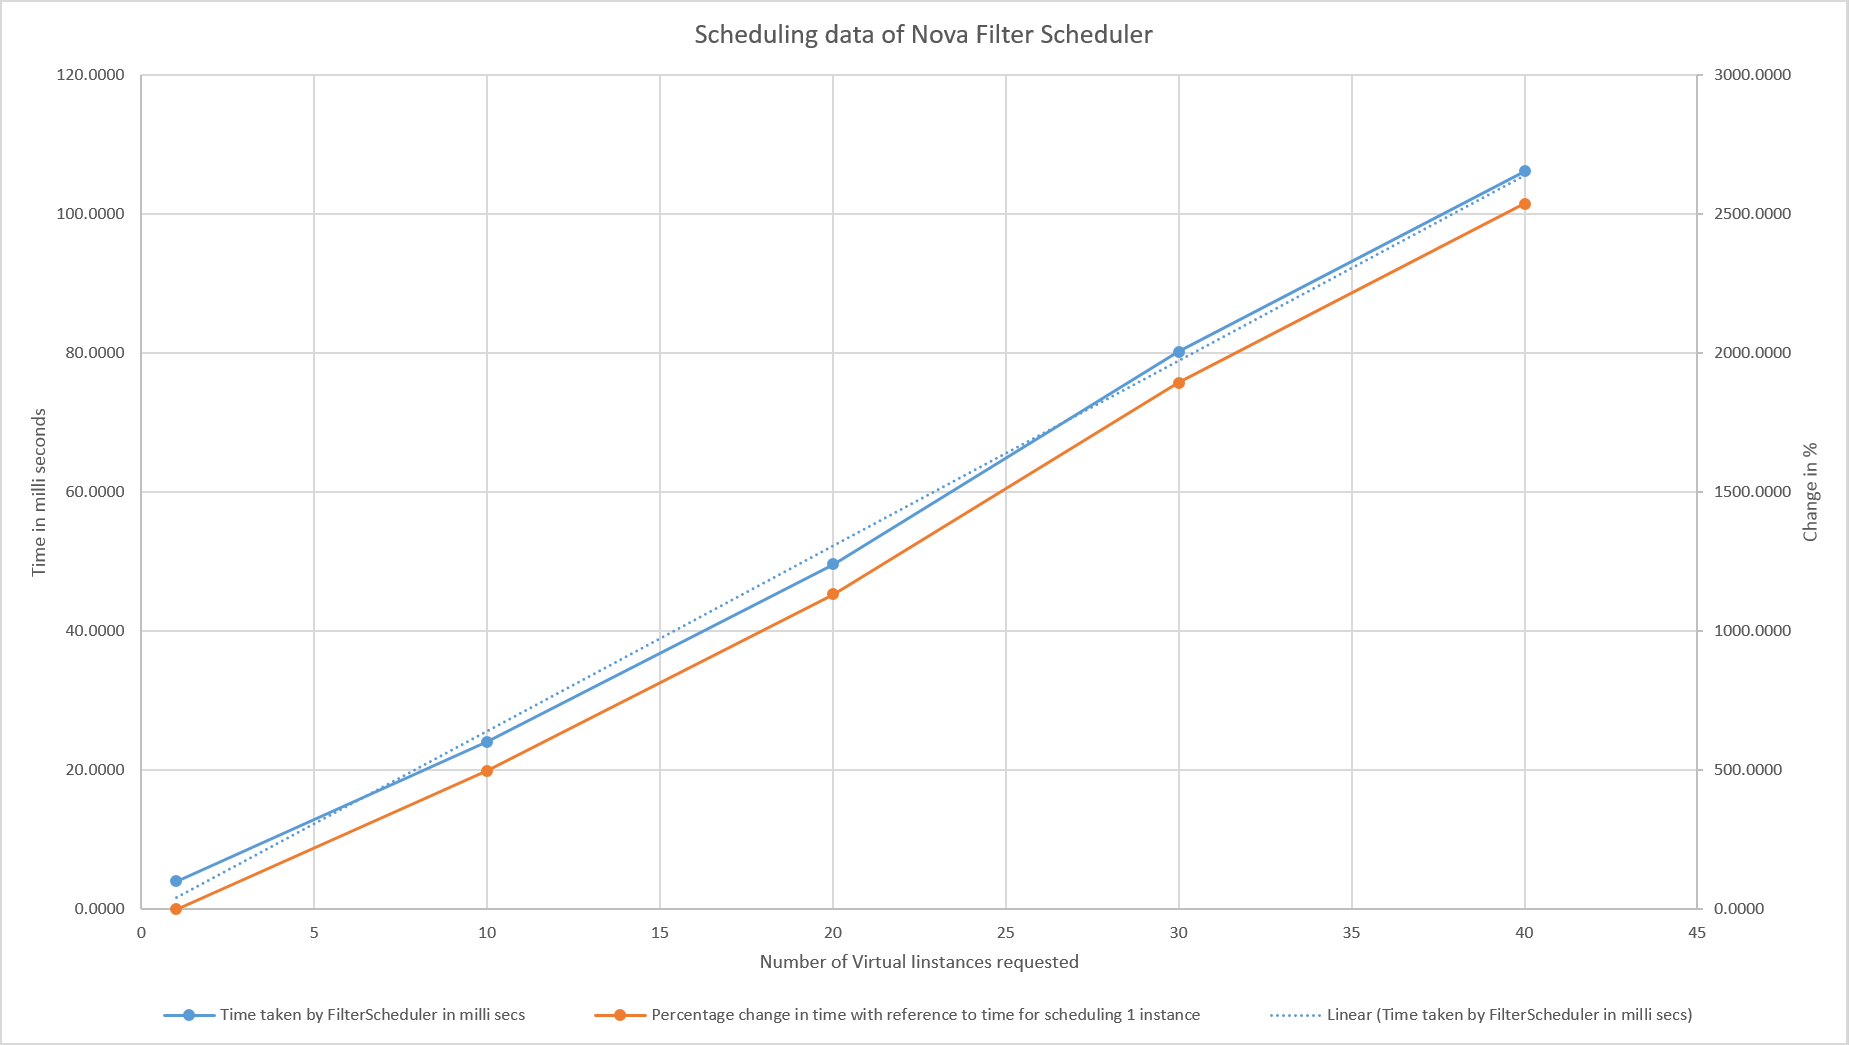
\includegraphics[width=1\linewidth]{NovaFilterSchedulerChart}
		\caption{Placement decision time for Standard Nova Scheduler from the data \ref{tabular:filterschedulerlogdata}}
		\label{fig:NovaFilterSchedulerChart}
	\end{center}
	\vspace{-10pt}
\end{figure}

The above table \ref{tabular:filterschedulerlogdata} is the time logs recorded for different requested number of virtual instances.
Here in the table, for providing a placement decision of 10 virtual instances, the standard nova scheduler takes around 24.10ms.
The percentage change in time is given by the change in time with reference to time for scheduling 1 instance.

\section{Observations of cPlex based scheduler}\label{sec:observationsoftucscheduler}

Observing the listing \ref{lst:tuc_schedule}, at the line \ref{line:tuc_get_filtered_hosts} it can be seen that the \verb|get_filtered_hosts| is executed only once for all the bulk requests of virtual instance scheduling.
This is followed by line \ref{line:solve_TUC_Cplex} \verb|solve_TUC_Cplex| to solve the scheduling problem for all the bulk requests.

In the log trace listing \ref{lst:tucschedulercodetracelog10vi} at the line number \ref{line:result_cplex_scheduler_placement}, it can be observed that, the placement decision of all the 10 virtual instances is concentrated on one host system \verb|"compute03"|.

The log trace listing \ref{lst:tucschedulercodetracelog10vi} provided in the Appendix \nameref{app:ch:logs} in chapter \nameref{app:sec:cplexschedulerlogtrace10vi} shows that only one instance of the \verb|get_filtered_hosts| is called to calculate the placement decision of 10 virtual instances.

\begin{figure}[H]
	\begin{center}
		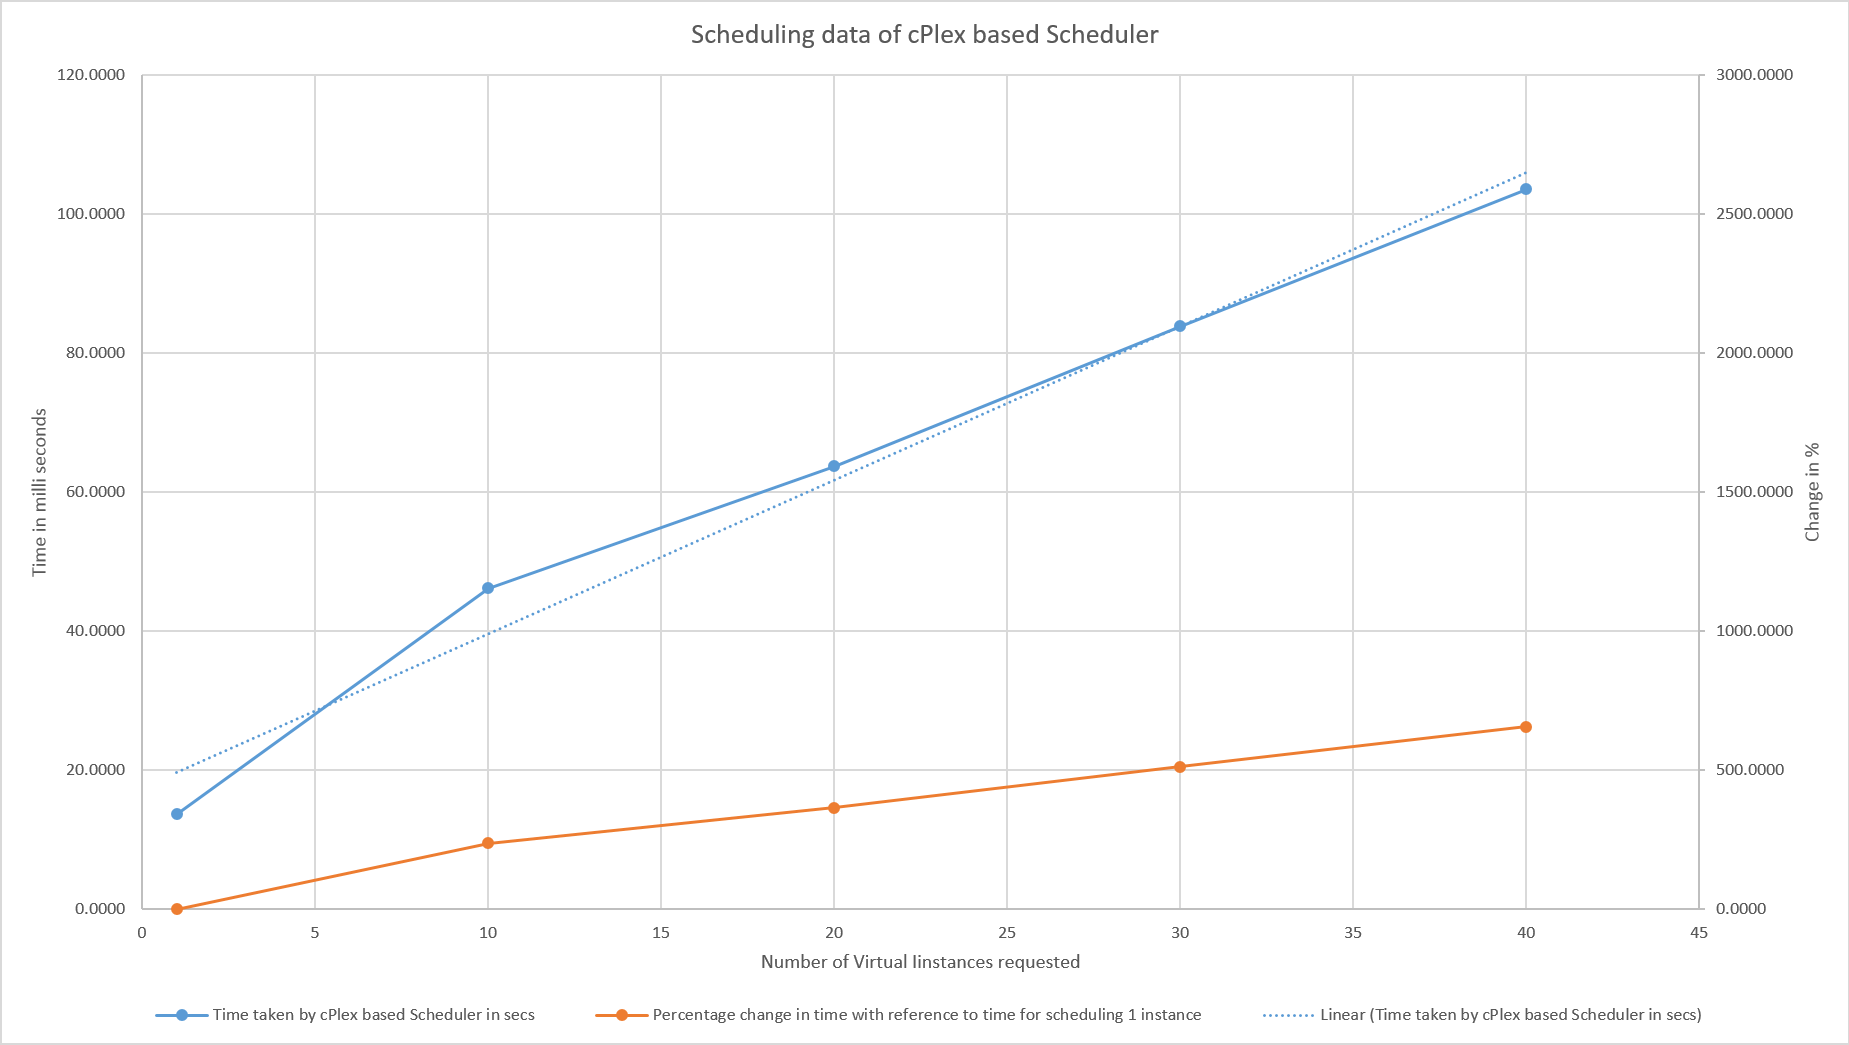
\includegraphics[width=1\linewidth]{cPlexSchedulerChart}
		\caption{Placement decision time for cPlex based Scheduler from the data \ref{tab:tucschedulerlogdata}}
		\label{fig:cPlexSchedulerChart}
	\end{center}
	\vspace{-10pt}
\end{figure}

\comment{
If the total requested capacity of RAM or HDD of virtual instances are more than the total available capacities, then the cPlex throws an exception as "unsolvable problem error". This exception is caught by the code and displayed as an error message on the screen.
}
\section{Comparision}\label{sec:comparision}

As stated in sections \nameref{sec:observationsofstandardnova} and \nameref{sec:observationsoftucscheduler}, the default Filter scheduler places the virtual instances across the hosts, whereas the \verb|tuc_ccn_scheduler| aggregates the creation of virtual instances on minimum possible host systems.
As the virtual instances on the new \verb|tuc_ccn_scheduler| are not spread across the multiple machines and aggregated on the few machines, the rest of the machines can be powered down which reduces the operating power costs.

On the other hand, combining the above two charts \ref{fig:NovaFilterSchedulerChart} and \ref{fig:cPlexSchedulerChart}, it can be observed that the slope of the cplex based scheduler is lesser than the slope of the standard nova filter scheduler. Which means that, for a larger requests of virtual instances, the cPlex based scheduler would be more efficient in providing the placement decisions for all the requested virtual instances. The initial offset time for execution of cPlex to solve the mathematical problem is higher compared to the standard nova filter scheduler.

\begin{figure}[H]
	\begin{center}
		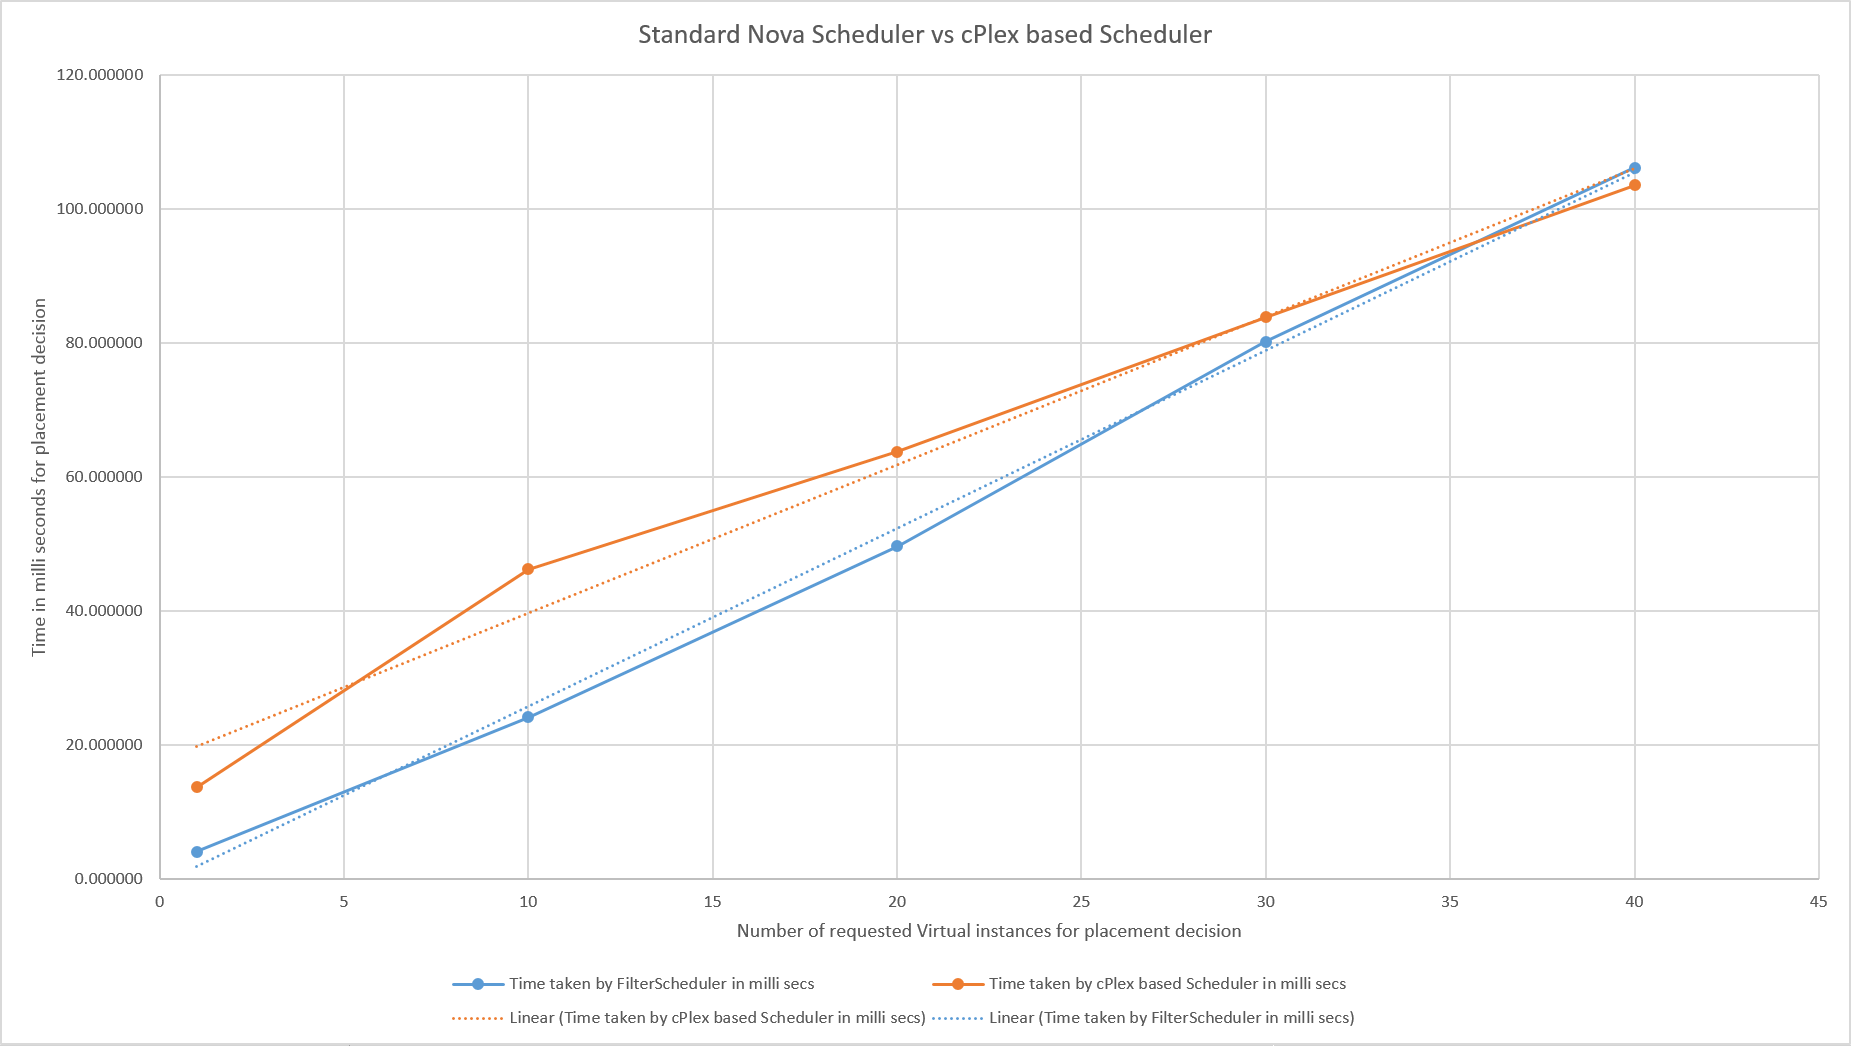
\includegraphics[width=1\linewidth]{novavscplex}
		\caption{Comparision of placement decision time between Standard Nova FilterScheduler and cPlex based Scheduler}
		\label{fig:novavscplex}
	\end{center}
	\vspace{-10pt}
\end{figure}

From the above chart \ref{fig:novavscplex}, it can be concluded that, the higher the number of requests to schedule the virtual instances the lesser the solving time for scheduling compared to the nova filter scheduler.

\section{Space for further improvements}\label{sec:spaceforimprovements}

As an example, let there be three host machines with a RAM capacity of 16GB each.
Let there be 9 virtual machines which consume 4GB of RAM each and shared equally among three host machines.
The available capacity of RAM is limited to 4GB on each machine whereas the total available capacity of RAM across all the machines is 12GB.
When there is a request for a virtual machine which requires the RAM of 8GB, both the schedulers would fail to make a placement decision for the requested virtual instance as there is no host with an available capacity of 8GB.

"Live Migration" is a functionality which would move the running virtual machine from one physical host machine to another physical host machine with minimum or no downtime.
Currently, the OpenStack Liberty has an ongoing issue with "Live Migration".
The live migration functionality fails to migrate the virtual instance from the source host machine to requested destination host machine and turns off the virtual instance scheduled for migration.
This "Live Migration" functionlity could mitigate the above mentioned issue with runtime reallocation of live(running) virtual machines to free the space by migrating it to any other possible hosts, freeing the space on the host and make a placement decision to allocate a new request of 8GB.

An idea for future could also be to have a shared resource pooling with a high speed dedicated networking bus on the hardware, to make the large clusters of compute servers into a single shared entity.